\section{Motivation}
\label{sec:motivation}

In this section, with help of a bank account example, we motivate the
need for a framework to express and enforce fine-grained
application-level consistency requirements under weak consistency
models. 
% \GK{The following text needs to be polished}

% We assume a system model where the eventually consistent database is organized
% as a collection of key-indexed, object-valued tables. The objects stored in the
% tables are instances of the same replicated data type. The database is composed
% of a number of \emph{replicas}, and each object is fully replicated across all
% the replicas. Under this model, a client request for an operation with no
% application-level consistency requirement can be serviced if at least one of
% the replicas is reachable. Thus, with the addition of new replicas, and placing
% them close to the clients, leads to improved throughput and reduced latencies.

\subsection{Bank account database}

Suppose our goal is to implement a highly available bank account
service on top of an eventually consistent data store. For the sake of
presentation, we restrict ourselves to bank account objects (records)
with following simple schema:

\begin{codesql}
Create Table BankAccount (
  accountNo int PRIMARY KEY,
  balance float CHECK (balance >= 0))
\end{codesql}

\noindent and with support for the following \emph{operations}:

\begin{codehaskell}
type AccountNo = Int
type Amount = Float
getBalance :: AccountNo -> Amount
deposit    :: AccountNo -> Amount -> ()
-- returns false if the account has insufficient balance
withdraw   :: AccountNo -> Amount -> Bool
\end{codehaskell}

\begin{figure}[t]
\centering
\subfigure[Unsafe Withdraw]{\label{fig:unsafeWithdrawAnomaly}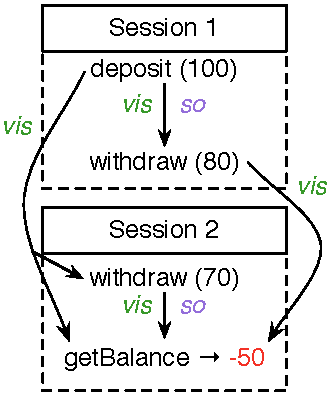
\includegraphics[width=0.31\columnwidth]{Figures/Motivation4}}
\hfill
\subfigure[Negative Balance]{\label{fig:negativeBalanceAnomaly}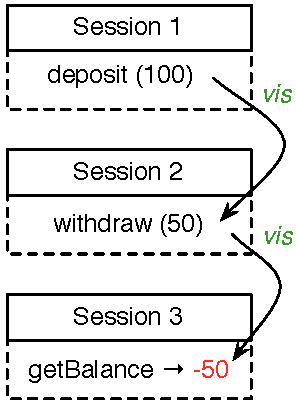
\includegraphics[width=0.31\columnwidth]{Figures/Motivation2}}
\hfill
\subfigure[Missing update]{\label{fig:missingUpdateAnomaly}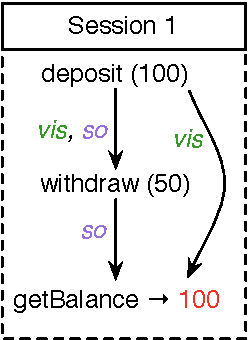
\includegraphics[width=0.26\columnwidth]{Figures/Motivation1}}
%\hfill
%\subfigure[Monotonicity violation]{\label{fig:monotonicityAnomaly}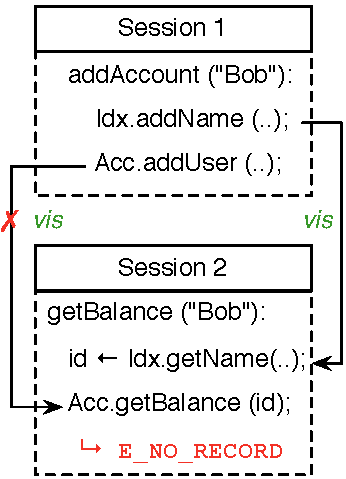
\includegraphics[width=0.36\columnwidth]{Figures/Motivation3}}
\caption{Anomalies possible under eventual consistency for the get balance operation.}
\label{fig:cleanliness_examples}
\end{figure}

The sole attribute of a \cf{BankAccount} object, identified by its unique
\cf{accountNo}, is its current \cf{balance}. A \cf{deposit} operation
on a \cf{BankAccount} adds some \cf{Amount} to its \cf{balance},
whereas a \cf{withdraw} operation subtracts. Operation \cf{getBalance}
returns the current \cf{balance} in the account. A \cf{withdraw}
operation succeeds and returns \cf{True} only if there is sufficient
balance in the account. Otherwise, it fails and returns \cf{False}. 

If we were to use a traditional database system to store
\cf{BankAccount} objects, all that needs to be done is to define the
\cf{BankAccount} schema, as shown above. The database management
system effectively sequentializes all accesses to the database, and
automatically enforces the required integerity constraints on the
data, so that it is never possible for a \cf{getBalance} operation to
return a negative balance, or for a \cf{withdraw} to succeed without
having sufficient balance in the account. However, under eventual
consistency, such anomalies are bound to occur as demonstrated in the
following subsection. 


\subsection{Anomalies}

Consider the execution shown in fig.~\ref{fig:unsafeWithdrawAnomaly}.
Assume that all operations in the figure are on the same
\cf{BankAccount} object with initial balance as 100. Execution
contains two concurrent client sessions, where one of the sessions
executes a \cf{withdraw} followed by a \cf{getBalance} operation. We
say that \c{withdraw} precedes \cf{getBalance} in \emph{session
order}, and visualize it as a directed \cf{so} edge from the former to
the later. Edges labelled \cf{vis} in the figure capture the
\emph{visibility} relation between operations; an operation is said to
be \emph{visible} to other operation if the later can witness the
effects of the former. Two operations that are not related either via
\cf{vis} or \cf{so} are said to be concurrent. The figure shows an
execution where concurrent \cf{withdraw}s in different sessions
succeed independently, but a subsequent \cf{getBalance} operation that
witnesses both the \cf{withdraw}s reports a negative balance. 

It is easy to see that the only way to ensure that integrity
constraint on \cf{balance} is to prevent concurrent withdrawls on the
\cf{BankAccount}. This can be done by insisting that \cf{withdraw} be
executed with strong consistency. Although this prevents unsafe
withdrawls from going through, a strongly consistent \cf{withdraw}
itself is not sufficient to prevent \cf{getBalance} from ever
reporting a negative balance to the end user.

Consider the execution shown in fig.~\ref{fig:negativeBalanceAnomaly},
which consists of three concurrent sessions performing a \cf{deposit},
a \cf{withdraw}, and a \cf{getBalance}, respectively, on the same
\cf{BankAccount}. Assume that initial balance in the account is zero.
As the \cf{vis} edge indicates, operation \cf{withdraw(50)} in session
2, can witnesses the effects of \cf{deposit(100)} from session 1,
leading it to rightfully conclude that the current balance is 100.
Consequently, \cf{withdraw(50)} is performed safely. The effect of
this \cf{withdraw} operation subsequently becomes visible to the
\cf{getBalance} in Session 3. However, \cf{getBalance}, which can only
see the effect of \cf{withdraw} from session 2, but not \cf{deposit}
from session 1, reports the balance of negative 50 to the user.

Negative balance is not the only inconsistency that the user is
exposed to under an eventually consistent bank account. Figure
~\ref{fig:missingUpdateAnomaly} shows an execution where
\cf{getBalance} operation in a session does not witness the effects of
\cf{withdraw} operation performed in the same session, possibly
because \cf{getBalance} was served by a replica that hasn't yet merged
the \cf{withdraw} effect, which could have been served by a different
replica. This anomaly leads the user to incorrectly conclude that the
\cf{withdraw} operation failed to go through.

Although it is easy to understand the reasons behind the occurance of
the aforementioned negative balance and missing update anomalies, the
fix is not quite apparent. Making \cf{getBalance} a strongly
consistent operation is definitely sufficient to avert anomalies, but
is it really necessary? Given that a strongly consistent operation is
significantly expensive, both in terms of latency and monetary value, we ideally
would not want to request strong consistency, unless there are
no alternatives available. Unfortunately, this requires us to
understand subtle differences in semantics of various kinds of weak
consistency alternatives, such as timeline consistency and session
guarantees, offered by off-the-shelf eventually consistent data
stores. This process is error-prone, and becomes further complicated
in presence of transactions, as demonstrated in Sec.
~\ref{sec:transactions}.


\subsection{Implementation in Quelea}

\name automates this error-prone task by letting the programmer
declare application-level consistency constraints as \emph{contracts}.
This obviates the need to understand store-level consistency guarantees,
and relieves the programmer from having to match application
requirements with appropriate store-level alternatives. The
cornerstone of declarative reasoning in \name is the programming model
that draws largely on the concept of operation-based
CRDTs~\cite{shapiroCRDT}. The state of a replicated data object in
\name is nothing but the set of effects applied on the object. For
example, to represent a \cf{BankAccount} object in \name, we first
define an sum type of all possible effects on a \cf{BankAccount}
object:
%types in Quelea are defined as reductions over the set of effects.
%The following data type definitions capture the operations and effects
%on the bank account and user index objects.
\begin{codehaskell}
type Amount = Float
data BankAccountEff = Deposit Amount
                    | Withdraw Amount 
                    | GetBalance
\end{codehaskell}
Subsequently, any \cf{BankAccount} object can be simply represented as a set of
effects of type \cf{BankAccountEff} that took effect on the object.
For example, a \cf{BankAccount} object obtained by performing a
deposit of 100 and a withdrawl of 50 on a fresh bank account is
represented as following:
\begin{center}
  \{\cf{Deposit(100), Withdraw(50)}\}
\end{center}
An operation on a replicated data object in \name is simply defined as
a reduction over the set of effects representing the object, and is
expected to produce a new effect along with a return value. For
instance, following are the definitions of operations on
\cf{BankAccount} type in \name (we represent sets as lists for
clarity):
\GK{Better define getBalance in terms of fold. It goes well with our
narrative.}
\begin{codehaskell}
type BankAccount = [BankAccountEff]
getBalance ::  BankAccount {- object -}
  -> () {- args -}
  -> (Amount {- ret val -}, 
      Maybe BankAccountEff {- effect -})
getBalance ctxt _ = (sum [v | Deposit v (- ctxt]
        - sum [v | Withdraw v (- ctxt], Nothing)

withdraw :: BankAccount -> Amount 
  -> (Bool, Maybe BankAccountEff)
withdraw c v = if fst (getBalance c ()) >= v
               then (True, Just (Withdraw v))
               else (False, Nothing)

deposit :: BankAccount -> Amount
  -> ((), Maybe BankAccountEff)
deposit _ v = ((), Just (Deposit v))
\end{codehaskell}

A \cf{getBalance} operation accepts a \cf{BankAccount} object
represented as a set of \cf{BankAccountEff}s, folds over the set
adding deposits and subtracting withdraws, and returns the resultant
amount, along with a new \cf{GetBalance} effect\footnote{wrapped
inside a \cf{Maybe} type for technical reasons}. A \cf{withdraw}
operation first checks if there is sufficient balance in the account.
If the check passes, it returns \cf{True} along with a new
\cf{Withdraw} effect. Otherwise, it returns \cf{False} and produces no
effect. The definition of \cf{deposit} can be similarly understood.

When a bank account operation is executed at one of the replicas in
response to a client request, \cf{BankAccount} object is constructed
using the effects available on the replica, and the definition of the
current operation is applied on the object. Note the set of effects
constituting the input \cf{BankAccount} object are the only effects
that are \emph{visible} to the current operation.  Formally, we say
that a \emph{visibility} relation exists between the input set of
effects and the newly engendered effect. In contrast, a concurrent
operation executing on a different replica can neither witness the
effect of the current operation, not can its effect be visible to the
current operation.

It is worthwhile to note that the above definitions of
\cf{BankAccount} operations are a straightforward encoding of the
expected behavior.  \name programming model provides the programmer
complete freedom regarding the semantics and desired convergence
property of the replicated data type, and indeed, we can encode the
well-known CRDTs~\cite{SSS} in a declarative fashion.  Observe that
the operation definitions presented here only capture the convergence
properties of the replicated data type, and are not concerned with the
consistency properties, which is expressed through the contract
language.

\subsection{Contracts}

We have previously observed that two \cf{withdraw} operations cannot
be executed concurrently for the integrity constraint on the account
balance to hold. Informally, this means that for any two distinct
\cf{withdraw} operations $a$ and $b$ on a \cf{BankAccount} object,
either the effect of $a$ must be visible to $b$, or the effect of $b$
must be visible to $a$. \name lets us declare this consistency
requirement as a contract over \cf{withdraw}:
\begin{smathpar}
\begin{array}{l}
\rsf{withdrawCtrt}(b) = \forall a. ~a \neq b \conj \rsf{isWithdraw}(a) \conj \\
\qquad \sameobj{a}{b} \Rightarrow \vis{a}{b} \vee \vis{b}{a} 
\end{array}
\end{smathpar}
The above definition of $\rsf{withdrawCtrt}$ is parameterized over the
effect ($b:\cf{BankAccountEff}$) generated by the \cf{withdraw}
operation. The predicate $\rsf{isWithdraw}$ is true for a
\cf{Withdraw} effect, and false for any other effect. $\sameobj{a}{b}$
is true if and only if $a$ and $b$ are effects over the same
\cf{BankAccount} object; we only require \cf{withdraw} operations on
same bank account to be totally ordered. Operations on other bank
accounts can be executed concurrently. Rest of the contract is a
straightforward translation of its informal presentation discussed
earlier. 

For the \cf{getBalance}, we construct a contract  precisely to prevent
the anomalies described previously. The contract is shown below:
\begin{smathpar}
\begin{array}{l}
\rsf{getBalCtrt}(c) = \forall (a,b). ~ \rsf{isDeposit}(a) \conj
  \rsf{isWithdraw}(b) \conj \\
\qquad \vis{a}{b} \wedge \vis{b}{c} \Rightarrow \vis{a}{c} \\
\qquad \vee (\soZ \cap \sameobjZ) (a,c) \Rightarrow \vis{a}{c} \\
\qquad \vee (\soZ \cap \sameobjZ) (b,c) \Rightarrow \vis{b}{c}
\end{array}
\end{smathpar}

\GK{It is better to split this contract into two parts.}
If a withdraw $b$ is visible to the get balance operation, then all
deposit operations $a$ visible to withdraw should be visible to the
get balance operation. This prevents negative balance anomalies. The
rest of the contract says that a get balance operation must witness
previous deposit and withdraw operations on the same object in the
same session. This prevents missed update anomalies.

Since the deposit operation does not have any restrictions, its
contract is simply $\true$.

Note that the above contracts for \cf{withdraw} and \cf{getBalance}
express their consistency requirements \emph{independent} of the
semantics of the underlying store. To write such contracts, a
programmer only needs to reason about the semantics of the application
under the replication model professed by \name. The mapping of
application-level consistency requirements to appropriate store-level
guarantees is done automatically behind the screen. This process is
described in the following two sections.
% Similar to contracts on operations, Quelea supports contracts on transactions.
% The contract on the \cf{getBalanceName} transaction is given below:
% \begin{smathpar}
% \begin{array}{l}
% \rsf{getBalanceNameCtrt} = \forall (a:\rsf{GetName}), (b:\rsf{GetBalance}), \\
% \quad (c:\rsf{AddName}), (d:\rsf{AddUser}). ~\trans{a}{b}{c}{d} \wedge \so{a}{b} \\
% \qquad \wedge ~\vis{c}{a} \wedge \sameobj{d}{b} \Rightarrow \vis{d}{b}
% \end{array}
% \end{smathpar}

% $\trans{a}{b}{c}{d}$ says that the action pairs $a,b$ and $c,d$ are in the same
% transaction, and the two transactions are distinct. The contract says
% specifically forbids the anomaly presented in
% Figure~\ref{fig:monotonicityAnomaly}. This is the desired semantics for the
% \cf{getUserName} transaction.

% The programmer simply defines such contracts on the operations and the
% transactions. Quelea logically analyzes the contracts, and maps the
% corresponding operation to the precise store consistency and isolation level.
% Thus, Quelea equips the programmer with a declarative model for reasoning and
% expressing eventually consistent programs.



